
\chapter{Empirical solar-wind model for the inner heliosphere}
\label{chap:empirical_solar_wind_model_for_the_inner_heliosphere}

The analyses in the previous chapter are focused on the solar wind's influence on the magnetosphere -- this chapter changes the main focus to the solar wind upstream of the magnetosphere, in a first step down to a solar distance of \SI{0.3}{\au} and then even further down to the region around \SI{10}{\Rs}, close to the solar wind's origin near the Sun. The solar wind's evolution on its way to \SI{1}{\au} from the near-Sun region is modeled with the goal of predicting the solar wind environment for the upcoming PSP mission.\\

context of motivation in thesis and paper introduction and context of results in thesis\\

%COFI -- chapter outline and flow integration
This chapter is constructed as follows, the PSP mission, its scientific goals, and the spacecraft are described, I introduce the analyses done in the publication \citet{Venzmer2017}, which is a major part of this chapter, an improvement to the magnetic field solar distance dependency is derived, which upgrades that from our article, other things, and further an outlook is given.\\


%%% contributions and copyright
The major part of this chapter is published as ``Solar-wind predictions for the Parker Solar Probe orbit'' in \citet{Venzmer2017} (replace arXiv cite with aanda's), which is referred to as 'the paper' in this work. The article, published in Astronomy and Astrophysics (A\&A), is included following this chapter, denoted as \autoref{chap:solar_wind_predictions_for_the_parker_solar_probe_orbit}, and \textbf{not yet} reproduced with permission, \textcopyright~ESO.

The analyses described in the paper were entirely done by me, as well as the tables, figures and equations. My coauthor Volker~Bothmer contributed to the text and the anonymous referee helped clarifying a few aspects. The text was further improved by the A\&A language editor Joshua~Neve.\\
% my own contributions to the paper (percentages):\\
% data analyses 100\\
% tables 100\\
% figures 100\\
% formulas 100\\
% section structure 80\\
% text 55\\
% - abstract 70\\
% - introduction 30\\
% - frequency distributions 65\\
% - solar activity dependence 70\\
% - solar distance dependency 60\\
% - empirical solar wind model 75\\
% - model extrapolation 35\\
% - discussion and summary 20\\


\section{Parker Solar Probe mission}

mission goals (see paper + \citet{Fox2015})\\
A photo of PSP during testing is shown in \autoref{fig:aa-roll-sc-into-acoustics-cell-0199} and an illustration of PSP flying near the Sun is shown in \autoref{fig:SPP_ObservingSun2}.\\
\begin{figure}[htb]
	\begin{floatrow}
		\ffigbox{
			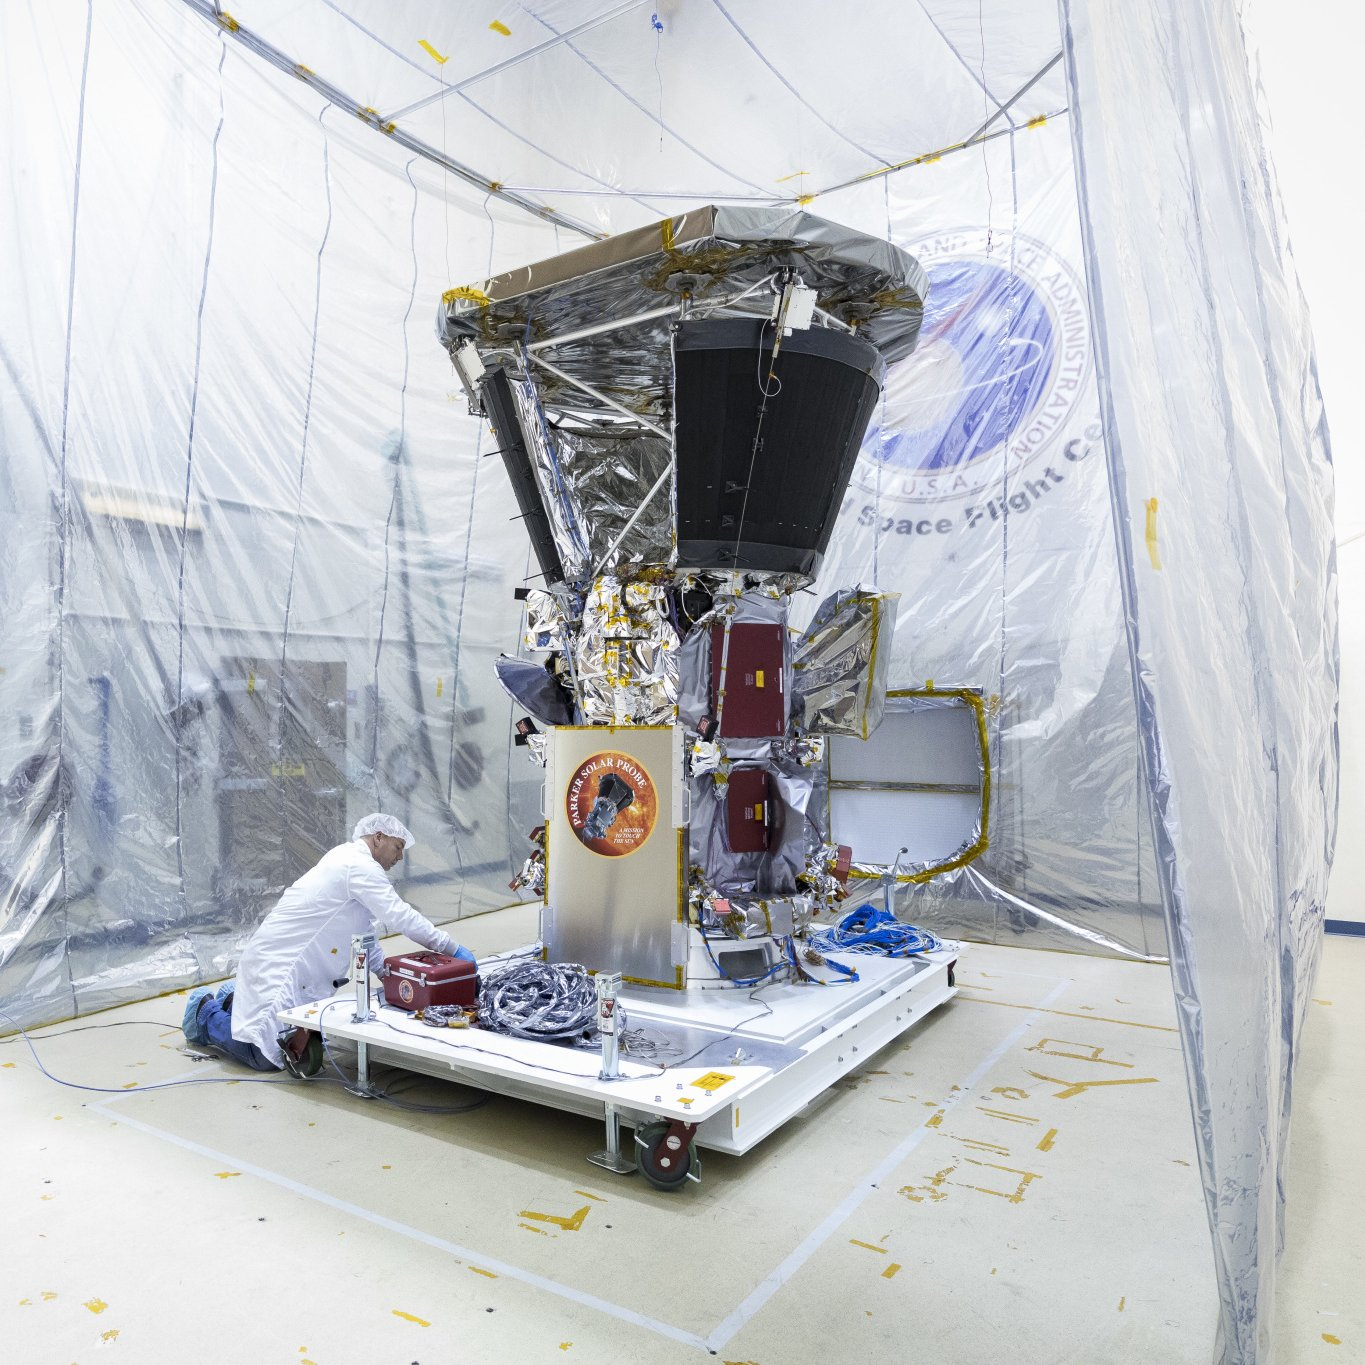
\includegraphics[width=0.5\textwidth]{images/aa-roll-sc-into-acoustics-cell-0199_square.jpg}
		}{
			\caption{PSP in the Acoustic Test Chamber at NASA’s Goddard Space Flight Center in November 2017. Credit: \href{http://parkersolarprobe.jhuapl.edu/News-Center/Show-Article.php?articleID=62}{NASA/Johns Hopkins APL/Ed Whitman}.}
			\label{fig:aa-roll-sc-into-acoustics-cell-0199}
		}
% http://parkersolarprobe.jhuapl.edu/News-Center/Show-Article.php?articleID=62
% http://parkersolarprobe.jhuapl.edu/News-Center/admin/Press-Releases/images/articles/aa-roll-sc-into-acoustics-cell-0199.jpg
		\ffigbox{
			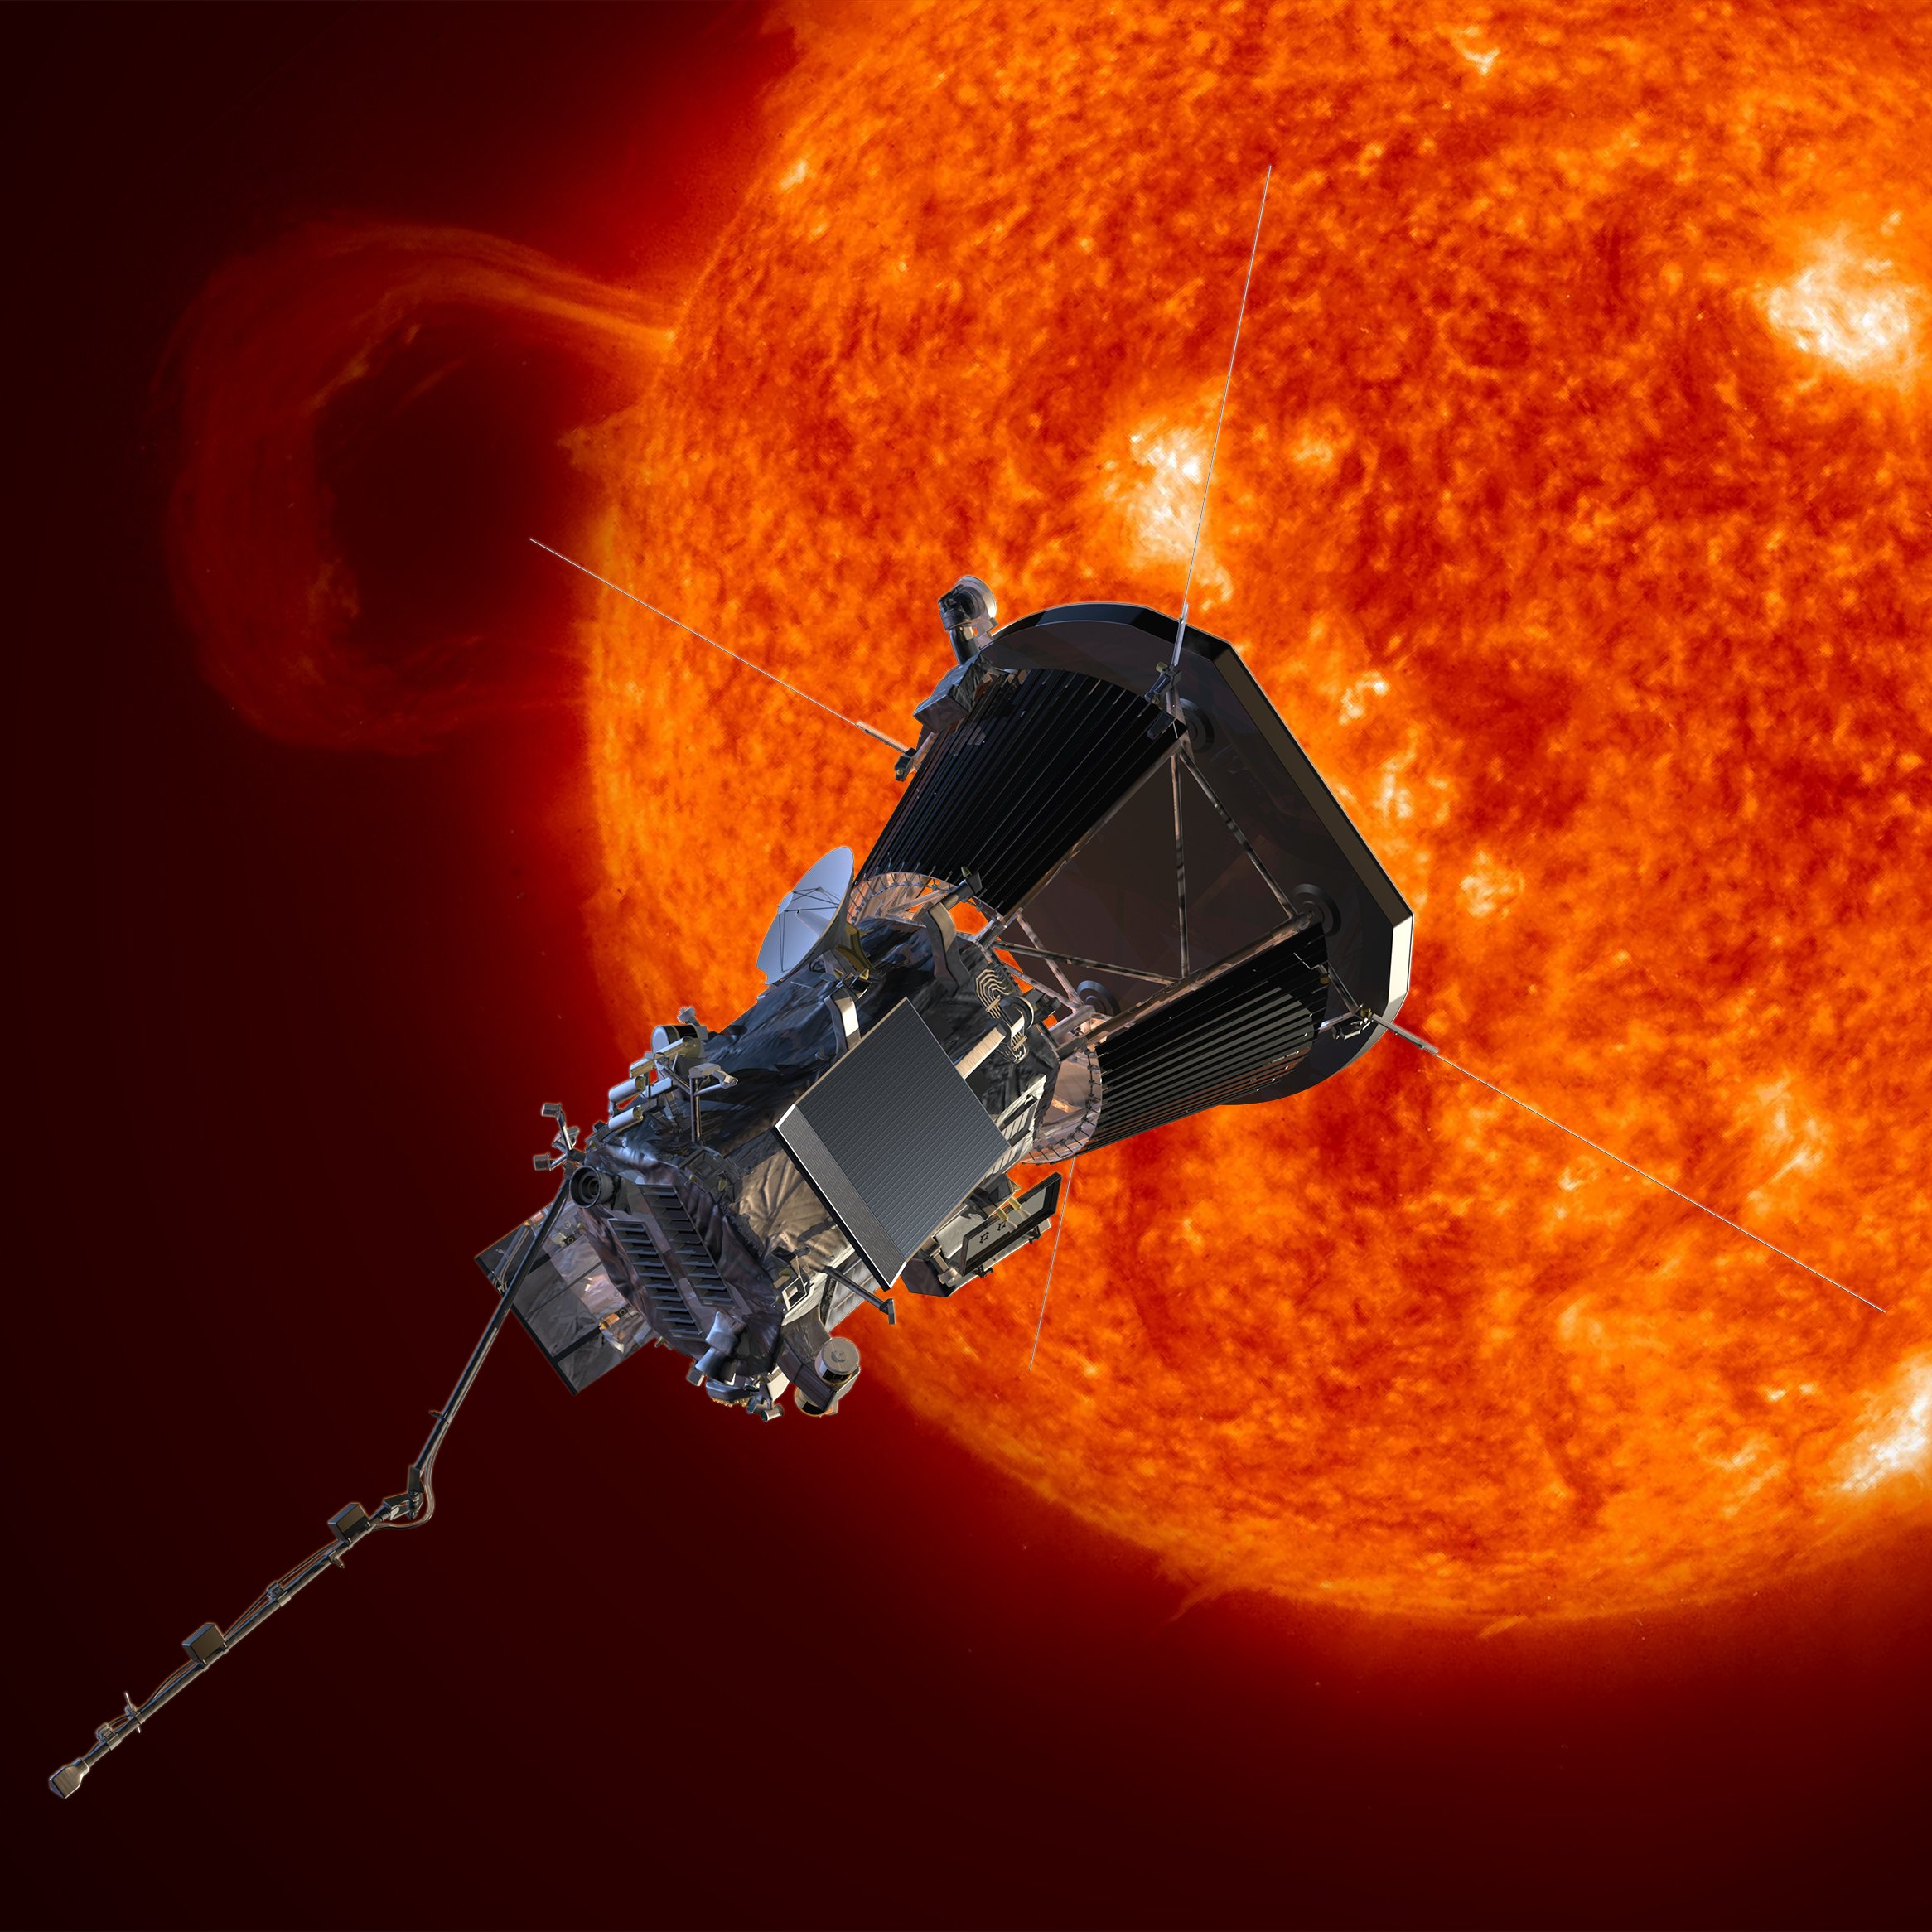
\includegraphics[width=0.5\textwidth]{images/SPP_ObservingSun2_square.jpg}
		}{
			\caption{Artist’s concept of PSP near the Sun. Credit: \href{http://parkersolarprobe.jhuapl.edu/Multimedia/Images.php}{Johns Hopkins University Applied Physics Laboratory}.}
			\label{fig:SPP_ObservingSun2}
		}
% http://parkersolarprobe.jhuapl.edu/Multimedia/ApprovedMedia/Images/Renderings/originals/SPP_ObservingSun2.jpg
% http://parkersolarprobe.jhuapl.edu/Multimedia/Images.php
		\end{floatrow}
\end{figure}

orbit figure? ref. to distance figure?\\
WISPR instrument\\
CGAUSS project -- context of this work in project objectives\\
Sun angular diameter comparison, see presi S³\\


\section{Paper content}
% from paper:
We obtained lognormal representations of the frequency distributions’ shapes of the four key solar wind parameters magnetic field strength, proton velocity, density and temperature. We derived analytical relations for the parameters’ solar activity dependencies and for their solar distance scaling. An empirical solar wind model was build from the combination of the obtained frequency distributions, SSN dependence relations and solar distance dependence functions, representing the solar wind’s solar activity and distance behavior. This empirical model was fed with SSN predictions and extrapolated to the orbit of PSP. We estimated solar wind median values during PSP’s first perihelion and modeled the values for PSP’s closest perihelia.\\

In order to derive the solar wind environment for the PSP orbit, finally the general solar wind model derived in the previous sections will be extrapolated to the PSP orbit, taking into account predictions of the SSN.\\


\subsection{Solar distance dependency---theory}
B-field radial profile: $B \propto r^{-1.5}$; exponent between -1 and -2\\
	Magnetic field model (Parker1958) (the equations are quoted in the next section)\\
velocity radial profile: $V \propto r^{0}$ (constant; Parker)\\
	maxwellian distribution? difference to lognormal...\\
density radial profile: $N \propto r^{-2}$\\
	simple view: For a spherical constant velocity mass outflow, a per distance squared law is expected, because of the mass flux conservation per solid angle for different distances. Measurements up to the outer heliosphere confirm the $r^{-2}$ dependency (1--38~au by Voyager~2, \citep{Belcher1993} newer paper?)\\

temperature radial profile: $T \propto r^{-1?}$\\
	at larger distances (specify...) heating outbalances the adiabatic temperature part (adiabatic cooling vs. pickup proton and stream--interaction heating; 1--68~au by Voyager~2; \citet{Richardson2003}\\
solar wind ram pressure $p_\text{ram} = \rho V^2$\\


\section{Improvement to the magnetic field solar distance dependency}
In our article, we scaled the magnetic field strength via a power-law function and obtained a solar-distance dependency proportional to $r^{-1.662}$. We also noted there that the model's near-Sun field magnitude, extrapolated to PSP's closest perihelion, will be lower than the actual values to be found. However, it was a simplified approach -- in the following I present a procedure, leading to an improved distance dependency, which also accounts for the contributions of the individual field vector components. The new distance dependency, extrapolated to the PSP orbit and combined with the solar activity dependency described in the paper, yields \SI{8}{\%} higher values at the first perihelion and \SI{32}{\%} higher values at the 22nd perihelion.\\

A more accurate distance dependency for the model is derived in the following.\\

The coronal magnetic field near the Sun rotates rigidly, holding on to the coronal plasma. At the solar-wind source surface (at around \SI{2.5}{\Rs}), where the thermal plasma pressure overcomes the magnetic pressure, the magnetic field gets radially transported outwards, maintaining only its radial vector component $\vect{B}_r$. From there on, the solar rotation begins to shear the magnetic field, building up a longitudinal component $\vect{B}_\phi$ as well. The solar-wind magnetic field model formulated by \citet{Parker1958} has the following components in spherical coordinates ($\theta$ is the colatitude):
\begin{align}
	\vect{B}_r(r) &= B_0 \left(\frac{r_0}{r}\right)^2 \cdot \vect{e}_r\,,\\
	\vect{B}_\phi(r) &= -B_0 \left(\frac{r_0}{r}\right)^2 \cdot \frac{\omega\,r\,\sin\theta}{v_\text{sw}} \cdot \vect{e}_\phi	\,,	\label{eq:b_phi_vector}\\
	\vect{B}_\theta(r) &= 0 \cdot \vect{e}_\theta\,.
\end{align}
$B_0$ represents the radial field component at the solar distance $r_0$. The solar surface equatorial angular rotation rate $\omega$ and the solar-wind velocity $v_\text{sw}$ are involved as well. From these equations it can be seen that $\vect{B}_r$ scales with increasing solar distance with $r^{-2}$, as it is expected for a spherical outflow, and $\vect{B}_\phi$ scales with $r^{-1}$ as expected for a two-dimensional point source. In-situ observations support the component's scaling according to these theoretical exponents, although in slow solar wind the scaling for $\vect{B}_\phi$ deviates somewhat from theory \citep{Mariani1978}.\\

From the magnetic field's absolute value
\begin{align}
	B(r) &= \sqrt{\vect{B}_r^2 + \vect{B}_\phi^2 + \vect{B}_\theta^2}\,,	\label{eq:B_absolute}\\
	B(r) &= \sqrt{\left(B_0 \left(\frac{r_0}{r}\right)^2\right)^2 + \left(-B_0 \left(\frac{r_0}{r}\right)^2 \cdot \frac{\omega\,r\,\sin\theta}{v_\text{sw}}\right)^2}\,,
\end{align}
it is apparent that the magnetic field strength does not scale with a simple power law. If the solar dipole axis tilt to the solar rotation axis is neglected and the radial field component $B_0$ is set to be in the equatorial plane at $r_0 = \SI{1}{\au}$, then $\theta = 90\degree$ and therefore
\begin{align}
	B(r) &= B_0 \cdot \sqrt{r^{-4} + \left(\frac{\omega\,r}{v_\text{sw}}\right)^2 r^{-4}}\,,	\label{eq:B_1au}
\end{align}
with the distance $r$ in units of [au].\\

%%% field angle phi %%%
The magnetic field angle in the solar equatorial plane is distance dependent and is calculated via
\begin{align}
	\phi_B(r) &= \arctan\left(-\frac{\omega \cdot r}{v_\text{sw}}\right)\,.
\end{align}
The angle becomes $\phi_B(\SI{1}{\au}) = \SI{-46.23}{\degree}$ when using the Sun's equatorial angular velocity $\omega_\text{eq} = \SI{14.37}{\degree\per\day}$ (for more details on solar rotation see appendix \autoref{sec:solar_surface_differential_rotation}) and the median solar-wind velocity $v_\text{sw} = \SI{416}{\km\per\s}$ from the paper.\\

During solar cycle minimum, the solar wind in the equatorial plane outside the source surface originates from polar regions at about \SI{+-60}{\degree} heliolatitude. This leads to a slightly underwound Parker spiral, because of the slower rotation rate at higher latitudes \citep{Banaszkiewicz1998}. Using the differential rotation rate $\omega(\SI{+-60}{\degree}) = \SI{13.69}{\degree\per\day}$ (see appendix \autoref{eq:omega_differential}), the field angle becomes $\phi_B(\SI{1}{\au}) = \SI{-44.84}{\degree}$.\\

Neglecting the solar rotation axis tilt to the ecliptic normal...\\

So, in the ecliptic at a solar distance of \SI{1}{\au}, the Parker spiral's observed magnetic field angle $\phi_B$ is centered most of the time at \SI{-45}{\degree} or in the opposite direction at \SI{135}{\degree}.\\

This is indeed measured at \SI{1}{\au} and is apparent from the angle's frequency distribution, using OMNI data of the time period 1963--2016, see \autoref{fig:histogram_B_angles_b}.\\
\begin{figure}[htb]
	\fcapside[\FBwidth]{
		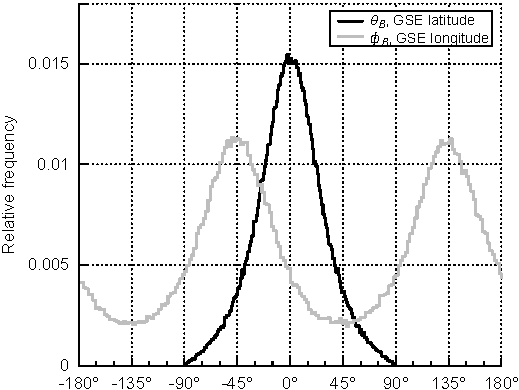
\includegraphics[width=0.6\textwidth]{images/gnuplots/histogram_B_angles_b.pdf}
	}{
		\caption{Frequency distributions of the magnetic field angles $\theta_B$ and $\phi_B$ in GSE coordinates. The frequencies are based on the hourly OMNI data during the period 1963--2016.}
		\label{fig:histogram_B_angles_b}
	}
\end{figure}

For $\phi_B$ being in average centered around these two directions, both vector components $B_r$ and $B_\phi$ have to be of equal amplitude. It can be seen from Equations~\ref{eq:B_absolute} and \ref{eq:B_1au} that this leads to
\begin{align}
	B(\SI{1}{\au}) &= B_0 \cdot \sqrt{2}	&\text{with}	&	&	\left(\frac{\omega\cdot\SI{1}{\au}}{v_\text{sw}}\right) &= 1\,.
\end{align}
However this way, $\omega$ and $v_\text{sw}$ are treated as constants and their variations with time are neglected.\\

%%% fit %%%
Considering the longitudinal field component, the magnetic field strength's distance dependency is derived in a similar way to that in the paper, see \autoref{sec:solar_distance_dependency}. Also, the same Helios data set is used for the fit as is in the paper.\\

In order to get an analytical representation of the radial dependence of the magnetic field, the function
\begin{align}
	x(r) = a \cdot \sqrt{\left(r^{e_1}\right)^2 + \left(r^{e_2}\right)^2}	\label{eq:sqare_power_law}
\end{align}
with the scaling parameter $a$, the exponents $e_1$ and $e_2$, is used in a least squares regression fit. From the theoretical considerations sketched above, the expected fit parameter values are: $a \approx \frac{B(\SI{1}{\au})}{\sqrt{2}}$, $e_1 \approx -2$, and $e_2 \approx -1$.\\

The resulting fit curves for mean and median field strength are plotted with respect to solar distance in \autoref{fig:radial_fit_B_thesis_skip}. In the Helios distance region \SIrange{0.3}{1.0}{\au}, the fit curves are very similar to those in the paper -- as they are expected to be. This is why this graph is visually almost indistinguishable to the corresponding one in the paper (paper \autoref{sec:solar_distance_dependency}, Figure~7).
\begin{figure}[htb]
	\fcapside[\FBwidth]{
		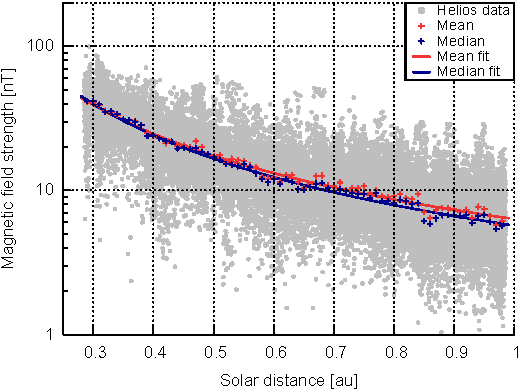
\includegraphics[width=0.6\textwidth]{images/gnuplots/radial_fit_B_thesis_skip.pdf}
	}{
		\caption{Magnetic field strength with respect to solar distance. The mean and median per \SI{0.01}{\au} data bin and their fit curves are plotted as well. The hourly Helios data has a native distance resolution of \SI{0.01}{\au}, thus, to make the distribution visible in this plot, I added a random distance value of up to \SI{+-0.005}{\au}.}
		\label{fig:radial_fit_B_thesis_skip}
	}
\end{figure}
The resulting fit parameters are presented in \autoref{tab:bfield_fit_parameters}\footnote{
%GUM statement
Concerning the error notation I adhere to the parentheses notation documented in the ``Guide to the expression of uncertainty in measurement'' (GUM) published by \citet{GUM2008}, where the numbers in parentheses are the errors on the corresponding last digits of the quoted value.
}.\\
\begin{table*}
	\caption{Fit parameter values for the curve fits (\autoref{eq:sqare_power_law}) and the distribution fit (eq XX), derived from the combined Helios~1 and 2 data. The numbers in parentheses are the errors on the corresponding last digits of the quoted value. The crossing distance indicates where the median and mean fits intersect each other. This distance is calculated numerically and that is why the error is only estimated.}
	\label{tab:bfield_fit_parameters}
	\centering
	\sisetup{table-figures-integer=1, table-figures-decimal=4, table-figures-exponent=0}
	\begin{tabular}{l l c c c c}
		\hline\hline
		\multirow{2}{*}{Fit}	&	&Factor	&\multicolumn{2}{c}{Exponents}	&Crossing distance\\
		\cline{4-5}
			&	&$a$	&$e_1$	&$e_2$	&[au]\\
		\hline
		\multirow{2}{*}{Curve}	&Median	&4.04(13)	&-1.852(25)	&-0.97(23)	&\multirow{2}{*}{0.336(10)}\\
			&Mean	&4.47(12)	&-1.740(18)	&-0.99(23)	&\\
		\multirow{2}{*}{Distribution}	&Median	&3.833(27)	&\multirow{2}{*}{-1.858(42)}	&\multirow{2}{*}{-1.32(12)}	&\multirow{2}{*}{--}\\
			&Mean	&4.081(29)	&	&	&\\
		\hline
	\end{tabular}
\end{table*}
%%% radial fit %%%
%4.47274*sqrt((r**-1.74028)**2 + (r**-0.990334)**2) = 4.04003*sqrt((r**-1.85224)**2 + (r**-0.974274)**2)\\
%r approx 0.336257719\\
%fit values
%4.04003	-1.85224	-0.974274
%4.47274	-1.74028	-0.990334
%errors
%0.130076	0.0246453	0.227053
%0.119049	0.0178415	0.228909
%table format
%4.04(13)	-1.852(25)	-0.97(23)
%4.47(12)	-1.740(18)	-0.99(23)
%avg WSSR = 27607.2	-6%
%med WSSR = 22254.7	-9%
%old avg WSSR = 29339.9	for simple power law function a*r^b
%old med WSSR = 24586.6
%
%%% fixed fit %%%
% 4.08078	-1.85771	-1.32237
% 3.83306	-1.85771	-1.32237
% errors:
% 0.0291872	0.042217	0.115887
% 0.0265236	0.042217	0.115887
% for table formatted:
% 4.081(29)	-1.858(42)	-1.32(12)
% 3.833(27)	-1.858(42)	-1.32(12)
% WSSR = 1.44202
% 1267.19055342511	this fit; is 33 % higher
% 950.841158464094	paper fit

Here, the WSSR slighly improved (\SI{6}{\%} for the median and \SI{9}{\%} for the mean) compared to the simple power-law function $x(r) = d \cdot r^e$ in \citet{Venzmer2017}. However, the mean and median fit curves still cross each other at a similar value as in the paper.\\

The obtained fit parameter values are similar to the theoretical values -- however, the larger exponent $e_1$ leads to a less steep slope near the Sun.\\

...and it can be fitted via a lognormal function\\

from paper:\\
'The mean and median velocity fit exponents acquired from the Helios data are very similar, which indicates that they can be kept identical so that the basic shape of the frequency distribution does not change with distance.

The crossing points limit the regions where the distribution's shapes can still be considered lognormal.

In order to still fit and extrapolate lognormal functions with the data, we assume that the shapes can be considered lognormal at all distances. For the frequency distribution fit function to be discussed in the following paragraph, we reduce the fit exponents $e_\text{med}$ and $e_\text{avg}$ to only one.

Implementing the power law distance dependency~(ref{eq:}) into the lognormal function (ref{eq:}), we get the fit parameters $d'_\text{med}$, $d'_\text{avg}$ and the common exponent $e'$.'\\


fix mean and median exponents and make a distribution fit. see fit distribution in \autoref{fig:fit_fixed_B_paper_f} and resulting fit parameters in \autoref{tab:bfield_fit_parameters}.\\
\begin{figure}[htb]
	\fcapside[\FBwidth]{
		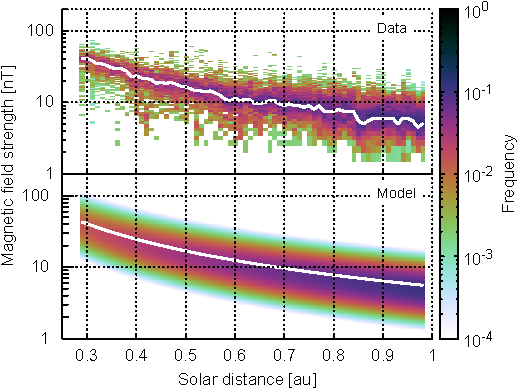
\includegraphics[width=0.6\textwidth]{images/gnuplots/fit_fixed_B_paper_f.pdf}
	}{
		\caption{Frequency distribution of the solar wind magnetic field strength with respect to solar distance. Plotted are the binned Helios data and the square-root power-law lognormal fit model with their median values (white lines).}
		\label{fig:fit_fixed_B_paper_f}
	}
\end{figure}

from paper:\\
'In order to estimate the solar-wind environment for the PSP orbit, we combine the results from the solar-wind frequency distributions’ solar-activity relationships and their distance dependencies derived from the OMNI and Helios data. The result is an empirical solar-wind model for the inner heliosphere which is then extrapolated to the PSP orbit in Sect.~ref{sec:}.'\\

The result of this analysis can be used to scale the SSN-relation derived in the paper:
\begin{align}
	B(ssn,r) = \frac{B(ssn)}{\sqrt{2}} \cdot \sqrt{\left(r^{e_1}\right)^2 + \left(r^{e_2}\right)^2}	\,.
\end{align}
The resulting equation, combined with the values obtained from the solar activity analysis in the paper \autoref{sec:solar_activity_dependence_of_the_solar_wind_frequency_distributions}, gives
\begin{align}
	B_\text{med}(ssn,r) &= \left(\SI{0.0131}{\nT} \cdot ssn + \SI{4.29}{\nT}\right) \cdot \sqrt{\left(r^{-1.86}\right)^2 + \left(r^{-1.3}\right)^2}	\,,\\
	B_\text{avg}(ssn,r) &= 1.0879 \cdot B_\text{med}(ssn,r)\,.
\end{align}

This magnetic field strength model is extrapolated to PSP's orbital range in \autoref{fig:sw_extrapolation_ssn_f}.\\
\begin{figure}[htb]
	\fcapside[\FBwidth]{
		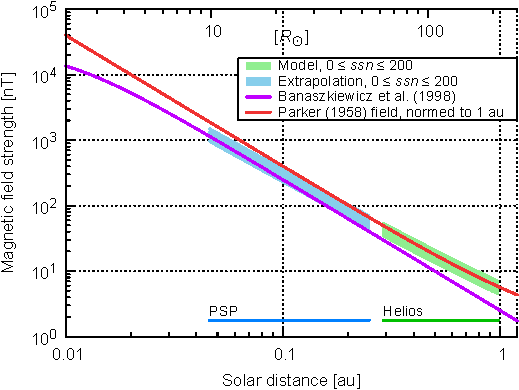
\includegraphics[width=0.6\textwidth]{images/gnuplots/sw_extrapolation_ssn_f.pdf}
	}{
		\caption{Radial extrapolation of the solar-wind magnetic field strength to the PSP orbit region. The median value from the model, obtained from Helios and OMNI measurements, is extrapolated to the PSP region for SSN values between solar minimum and maximum, that is, $0 \le ssn \le 200$. The lower edges of the shaded areas correspond to solar minimum, the upper edges to solar maximum. Also plotted are the radial dependencies of the analytic DQCS magnetic field model for solar minimum (violet) from \citet{Banaszkiewicz1998} and the Parker field model (red).}
		\label{fig:sw_extrapolation_ssn_f}
	}
\end{figure}

forecast to PSP orbit and mission time, see \autoref{fig:PSP_perihelia_prediction_f}\\
\begin{figure}[htb]
	\fcapside[\FBwidth]{
		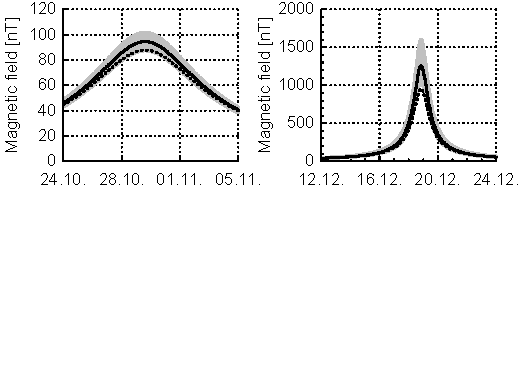
\includegraphics[width=0.6\textwidth]{images/gnuplots/PSP_perihelia_prediction_f.pdf}
	}{
		\caption{Estimated solar-wind parameter medians (solid) and their error bands (gray area) during 12~days in 2018 and 2024 with PSP's first perihelion at about \SI{0.16}{\au} and PSP's 22nd (the first closest) perihelion at \SI{0.046}{\au}. The prediction from \citet{Venzmer2017} is indicated as well (dotted).}
		\label{fig:PSP_perihelia_prediction_f}
	}
\end{figure}
% first perihelion value:
% 94 nT	this fit; is 8 % higher
% 87 nT	old fit
% first closest perihelion value:
% 1241 nT	this fit; is 32 % higher
% 943 nT	old fit

The estimated magnetic field strength median value of \SI{94}{\nano\tesla} for the first perihelion is \SI{8}{\%} higher than that in the paper. However, the median value of \SI{1241}{\nano\tesla} for the first closest perihelion is \SI{32}{\%} higher.\\


The estimated frequency distributions of the solar-wind magnetic field strength at PSP's 1st and 22nd (first closest) perihelion are plotted in \autoref{fig:PSP_sw_distributions_b}.\\
\begin{figure}[htb]
	\fcapside[\FBwidth]{
		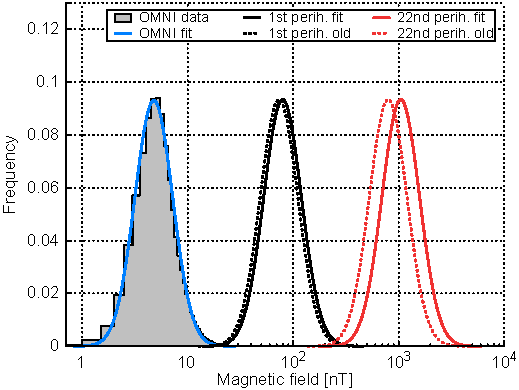
\includegraphics[width=0.6\textwidth]{images/gnuplots/PSP_sw_distributions_b.pdf}
	}{
		\caption{Frequency distributions of the solar-wind magnetic field strength (OMNI data) and those estimated with the solar-wind model for PSP's 1st and 22nd (first closest) perihelion. In this plot the frequencies of both extrapolated curves are scaled for visibility to the same height as the \SI{1}{\au} distribution. The predictions from \citet{Venzmer2017} are indicated as well (dotted).}
		\label{fig:PSP_sw_distributions_b}
	}
\end{figure}

%conclusion
The newly derived dependency relation can be used to replace that found in the paper.\\


\section{Outlook}
Currently, the solar-wind model described in this chapter is purely empirical and its four solar-wind quantities are characterized independently from each other. Now in further steps, theoretical relations connecting the parameters could be introduced to make the model self-consistent. For example, flux conservation could be implemented into the radial distance dependencies, relating the two parameters density and velocity (see section~XX), and also the velocity within the magnetic field's $\vect{B}_\phi$-component (\autoref{eq:b_phi_vector}) could be respected as a variable (not as a constant as it is done in the previous section).\\

PSP's in-situ measurements, starting in fall 2018, will eventually reveal how accurate the predictions of this model are.\\

Data captured from spacecraft that studied Mercury (perihelion distance of \SI{0.3}{\au}), such as Mariner~10 and MESSENGER, could be included to refine the distance dependency of the solar-wind model.\\
%MESSENGER: B-field 2004--2011

- further investigations should be done into structure extrapolations\\
- outward extension of model seems feasable (e.g., to Mars)\\


\subsection{flux conservation}
conserved quantities:\\
- momentum conservation... VBbookp112\\
- flux conservation...\\

%%%%%%%%%%%--  flux  --%%%%%%%%%%%%%%%
%As Schwenn1983 stated ``From Helios in situ measurements we know that at least beyond 0.29~au there is almost no nonradial flow, on the average. In fact, the particle flux was found to be that quantity which varies the least with increasing R.''\\

%Schwenn1990:
%increase in sw velocity with distance; speed increase mainly in slow solar wind
%density deviates from a purely r^-2 fall-off (10% faster); n(r)=6.1*r^-2.1 cm^-3; different behavior in slow and fast wind
%proton flux density constant between 0.3-1.0~au -> no meridional flow into/out of the ecliptic; different for slow and fast sw

With consideration of continuity, the mass flux per solid angle has to be constant: $\dot{m} = \text{const}$\\
conserved quantities:\\
- mass flux: $\dot{m} = \rho v A$ (with mass density $\rho$, velocity $v$ and solid angle A)\\
- particle fluxes (proton flux, electron flux, etc.)\\
	- proton flux: $j_\text{p} = n_\text{p} v_\text{p} A$ (with proton density $n_\text{p}$ and proton velocity $v_\text{p}$)\\

(with proton mass density $\rho = n_\text{p} m_\text{p}$ (with proton number density $n_\text{p}$ and proton mass $m_\text{p}$).)\\

the individual radial dependencies for a spherical radial outflow are:\\
$A(r) \propto r^2$ --> $A/r^2 = \text{const}$\\
and assuming an exponential dependency,\\
$n_{\text{p}}(r) = n_0 r^{c_n}$,\\
$v(r) = v_0 r^{c_v}$\\
\begin{align}
	j_\text{p} &= \text{const}\\
	n_\text{p} v_\text{p} A &= \text{const}\\
	n_0 r^{c_n} v_0 r^{c_v} r^2 &= \text{const}\\
	r^{c_n} r^{c_v} r^2 &= \text{const}\\
	\Rightarrow c_n + c_v + 2 &= 0\\
	c_n + c_v &= -2
\end{align}
an increasing velocity should result in a steeper density...\\

validity of mass flux continuity: within the heliosphere mass to energy conversion and vice versa is negligible, but there can be flux from and to higher latitudes as the Helios data is localized to a small latitude range in the ecliptic plane.\\
larger errors should be located near CMEs and CIRs (nonradial flows from interactions)\\
there is a proton flux difference between slow and fast solar wind streams (see book Schwenn1990 p.~146)

estimate the possible size of error:\\
(constant mass flux only for mean)\\
$c_n = -2.114$\\
$c_v = 0.0990$\\
$c_n + c_v = -2.024$\\
difference to -2 is 0.024\\



\section{Literature}
Schwenn1983 intro -> sw-averaging comment (beer and wine) (cite him...)\\
see Hellinger2013 p.1353\\
see astro70/CGAUSS/dropbox\_presis/... (presi 1.07 Inside Helios-Origins and Evolution-Salem.ppt -> Helios reloaded; radial functions for all parameters)\\
see Balogh1999 from p. 162 (Helios CIR results)\\
see Marsch1999... (model constraints)\\
On solar wind acceleration and SPP proposition: McComas2007\\
Parker1963 book, p.~75 -> isothermal expansion figure\\	%https://babel.hathitrust.org/cgi/pt?id=uc1.b4264142;view=1up;seq=12

Motivational question: What is the evolution of the solar wind parameters/structures before arriving at Earth?\\
what is meant by the term evolution?\\


\section{Seasonal solar wind variations}
seasonal variation by month\\
quantify variation amplitudes\\

see \autoref{fig:OMNI_monthly_freq_V_gps}
\begin{figure}[htb]
	\centering
	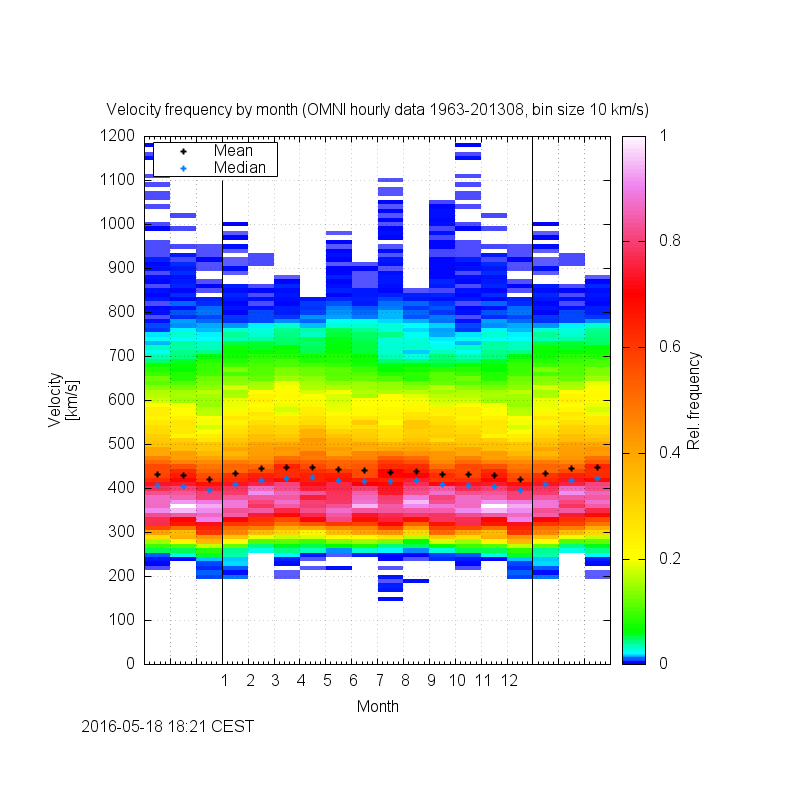
\includegraphics[width=0.3\textwidth]{images/gnuplots/OMNI_monthly_freq_V_gps.png}
	\caption{Diagram of the velocity frequency by month for the period 1963/01--2013/08. Mean and median values are shown as well.}
	\label{fig:OMNI_monthly_freq_V_gps}
\end{figure}

see \autoref{fig:OMNI_monthly_freq_B_a_gps}
\begin{figure}[htb]
	\centering
	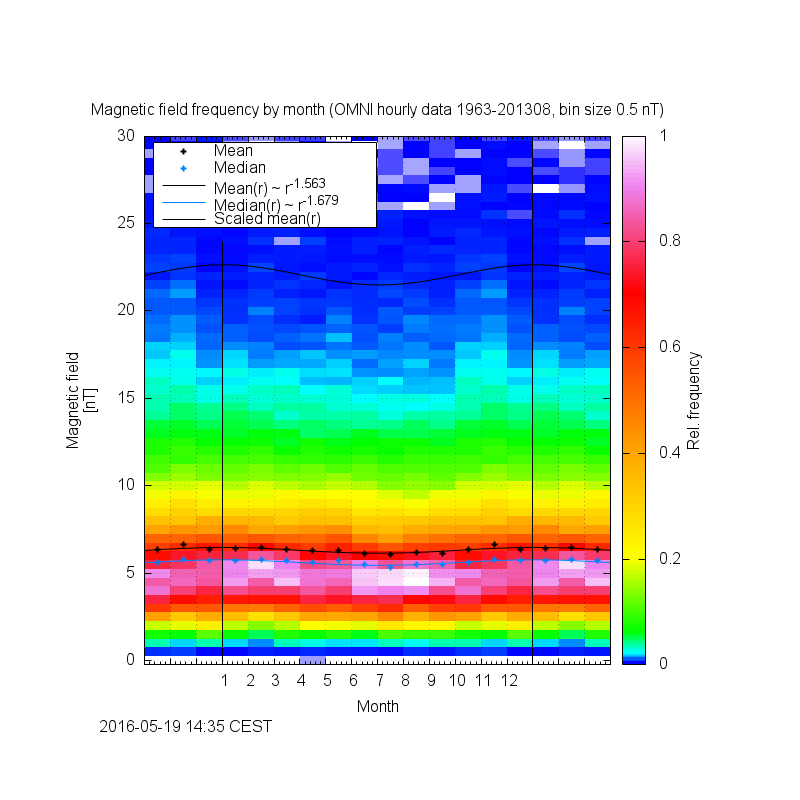
\includegraphics[width=0.3\textwidth]{images/gnuplots/OMNI_monthly_freq_B_a_gps.png}
	\caption{Diagram of magnetic field frequency by month for the period 1963/01--2013/08. Mean and median values are shown as well as the expected course from the solar distance variation (obtained from Helios data).}
	\label{fig:OMNI_monthly_freq_B_a_gps}
\end{figure}

derived exponent values from simple trigonometric fit on monthly values:\\
$c_n = -2.234$\\
maybe figure?\\

expected influence from Earth's perihelion/aphelion (see Appendix...) distance vs observations\\
we expect for the mean proton density (scaling law $n(r) \propto r^{-2.114}$):\\
$n(0.983~au) = 7.098~cm^{-3}$\\
$n(1~au) = 6.845~cm^{-3}$\\
$n(1.017~au) = 6.605~cm^{-3}$\\
we expect for the magnetic field strength (paper scaling law $n(r) \propto r^{-1.662}$):\\
$B(0.983~au) = 5.870~nT$\\
$B(1~au) = 5.705~nT$\\
$B(1.017~au) = 5.547~nT$\\


\section{Latitude dependency}
refer to Ulysses \autoref{fig:McComas2008_Ulysses_orbit}\\
Ulysses swoops polar plots...\\

see Schwenn1990's~Fig.~3.14\\
see also \citet{Schwenn1990} p.~127\\
see also \citet{Richardson1995}\\
Balogh et al. (1999) p. 162 ff (origin and formation of CIRs in inner heliosphere with Helios data; latitude V dependence)\\

Helios latitude; see \autoref{fig:latitude_frequency_4_thesis_plot}
\begin{figure}[htb]
	\centering
	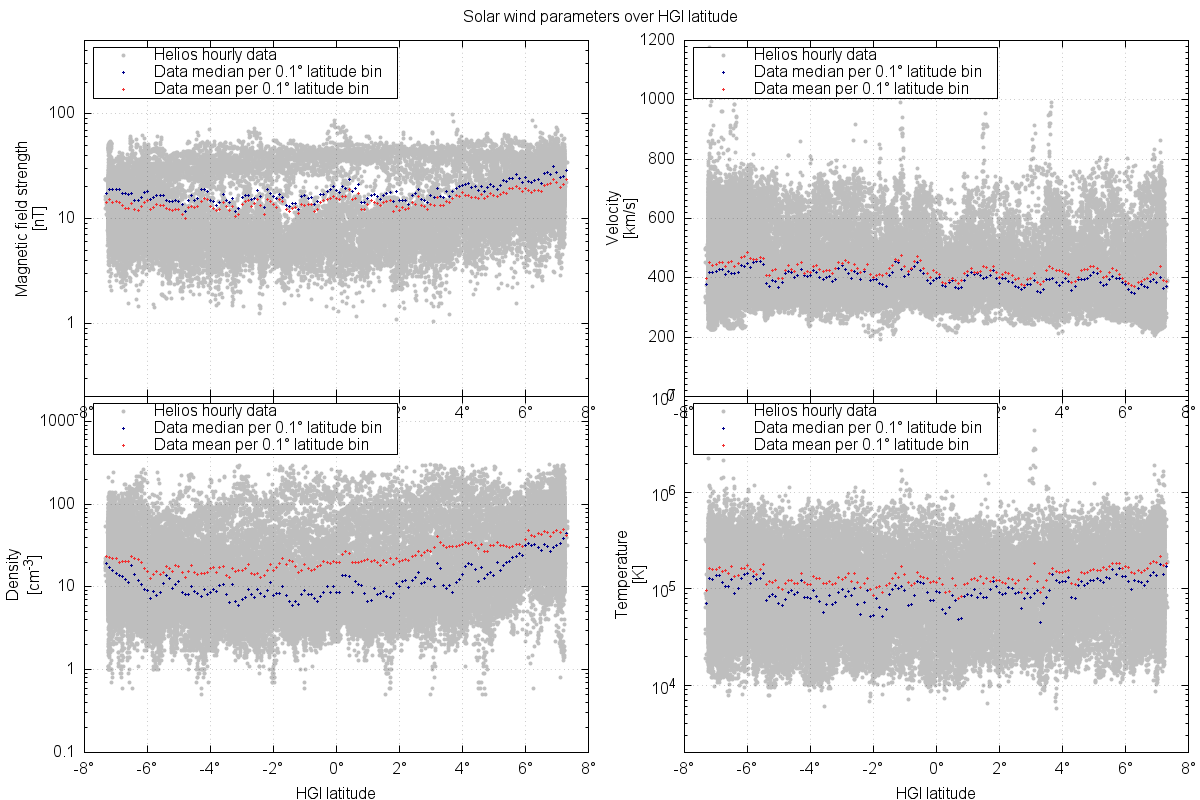
\includegraphics[width=0.5\textwidth]{images/gnuplots/latitude_frequency_4_thesis_plot.png}
	\caption{The four solar wind parameter's HGI latitude dependency. Their mean and median values per \SI{0.1}{\degree} bin are plotted as well. random jitter...}
	\label{fig:latitude_frequency_4_thesis_plot}
\end{figure}

with the exponential dependencies to 1~au projected solar wind parameters; there are only small changes with latitude in the range \SIrange{-7.25}{7.25}{\degree}\\
have a look on distribution widths...\\

dependence from latitude in interval \SIrange{-7.25}{7.25}{\degree} in Helios data negligible?, see \autoref{fig:latitude_frequency_rcorrected_v3_4_thesis_plot}.\\
\begin{figure}[htb]
	\centering
	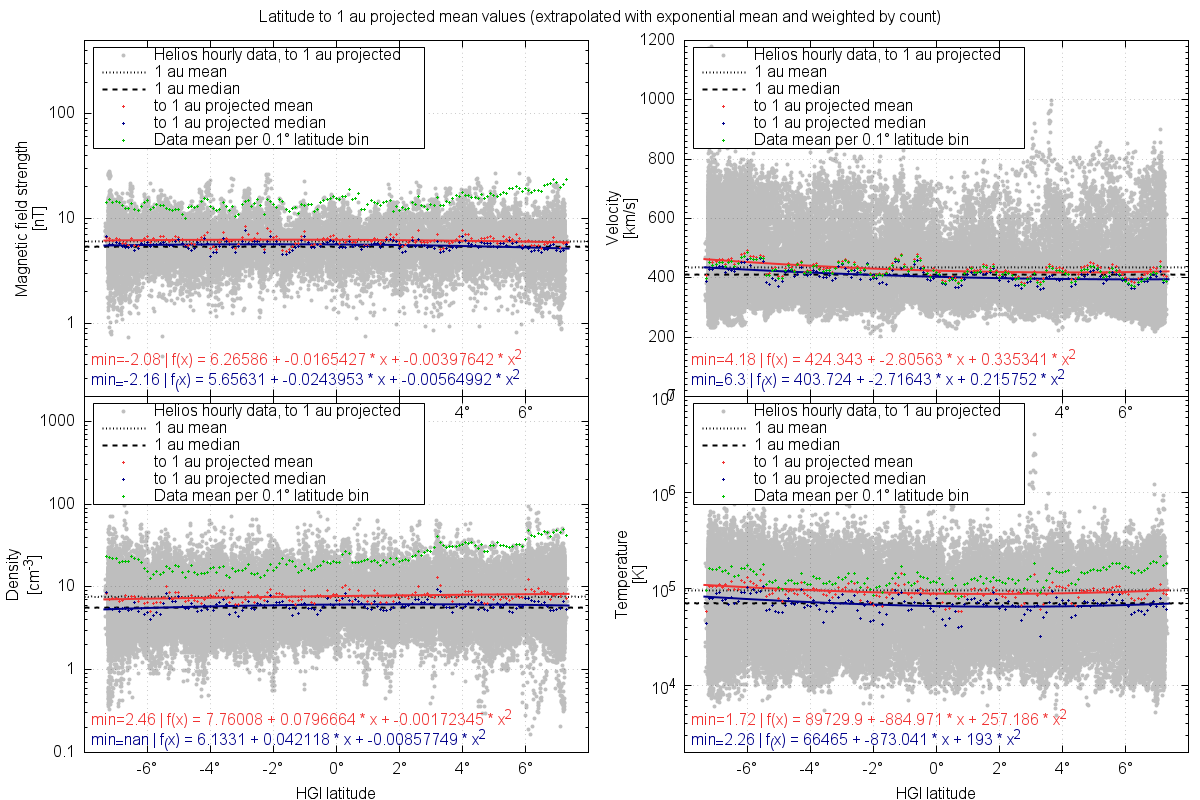
\includegraphics[width=0.5\textwidth]{images/gnuplots/latitude_frequency_rcorrected_v3_4_thesis_plot.png}
	\caption{Solar wind parameters projected to 1~au with respect to latitude. And their mean values, including weighted fit. add projected median... random jitter...}
	\label{fig:latitude_frequency_rcorrected_v3_4_thesis_plot}
\end{figure}
estimate error ranges from latitude influence...\\

...plot Ulysses data into plot?\\

%latitude variation negligible?
influence from latitude variation in data negligible? (see Ulysses \autoref{fig:McComas2008_Ulysses_orbit} in introduction). Helios probes within ecliptic => variation span equal to solar tilt: \SIrange{-7.25}{7.25}{\degree}; solar tilt/obliquity to ecliptic: $i_\odot = 7.25\degree$ (Sun fact sheet: \url{http://nssdc.gsfc.nasa.gov/planetary/factsheet/sunfact.html)}\\
big part of Helios data is from latitudes $>\pm5$°, see Figure~XX (data count over latitude) and see \autoref{fig:Helios12_orbits_ecliptic_polar} (Helios orbit polar plane in data section)\\


\section{Radial evolution of solar wind structures}
%see CGAUSS report2015_2

Helios event lists HSSs, SLOWs, CIRs, CMEs...; event lists for all Helios data\\
see Liu2004 for Helios ICME list and radial dependencies of $B$, $n$, $T$ and $v$...\\

\SI{200}{\km\per\s} slow solar wind at \SI{10}{\Rs} is in agreement with blob measurements from Wang2000\\

very slow sw (VSSW) gets accelerated; see Sanchez-Diaz2016:\\
%"The reported in situ measurements suggest that the properties of VSSW are a continuation of the slow wind toward lower speeds: higher densities, higher proton fluxes, and lower temperatures, thereby extending well-known scaling laws [Lopez and Freeman, 1986; Hundhausen et al., 1970] down to speeds as low as 200 km/s."\\
%"The VSSW has a number of interesting properties that suggest it may be the interplanetary signature of long HPS crossings."\\


radial diameter of MCs increase between 0.3~au and 4.3~au proportional to the distance as $r^{0.8}$ \citep{Bothmer1998}\\
MC central axial magnetic field strength radial density dependence $B = 18.1\,r^{-1.64}$ \citet{Leitner2007}\\
MC average diameter $D = 0.23\,r^{1.14}$ \citet{Leitner2007}

sw structure marked plots\\

structure extrapolations\\


